\documentclass[10pt]{beamer}

\usepackage[utf8x]{inputenc}
\usepackage[OT4]{fontenc}

\usepackage[polish]{babel}

\setbeamertemplate{navigation symbols}{}

\usetheme[bullet=circle,
          titleline=true,
          pageofpages=z,
          alternativetitlepage=true]{Torino}

\usepackage{ragged2e}
\usepackage{hyphenat}
\usepackage{hyperref}
\usepackage{booktabs}
\usepackage{listings}
\usepackage{multibib}
\usepackage{multicol}

\usepackage{tikz}
\usepackage{pgfplots}

\usetikzlibrary{arrows}
\usetikzlibrary{automata}
\usetikzlibrary{backgrounds}
\usetikzlibrary{decorations}

\usepackage{amsmath}
\usepackage{amsfonts}
\usepackage{amsthm}

\usepackage{pythonhighlight}

\title{SymPy --- czyli matematyka w Pythonie}
\author{Mateusz Paprocki \texttt{<mattpap@gmail.com>}}
\institute{Continuum Analytics, Inc.}
\date{\today}

\setbeamercovered{transparent}

\begin{document}

\begin{frame}[plain,t]
    \maketitle
\end{frame}

\begin{frame}[fragile]
  \frametitle{XXX}
  \framesubtitle{}

  \begin{python}
    In[1]: import math
    In[2]: math.sqrt(3)
  \end{python}
  \begin{equation*}
    1.7320508075688772
  \end{equation*}

  \begin{python}
    In[3]: import sympy
    In[4]: sympy.sqrt(3)
  \end{python}
  \begin{equation*}
    \sqrt{3}
  \end{equation*}

  \begin{python}
    In[5]: _4.evalf()
  \end{python}
  \begin{equation*}
  1.73205080756888
  \end{equation*}

  \begin{python}
    In[6]: _4.evalf(n=50)
  \end{python}
  \begin{equation*}
    1.7320508075688772935274463415058723669428052538104
  \end{equation*}
\end{frame}

\begin{frame}{Możliwości}
  \begin{multicols}{2}
    \tiny
    \begin{itemize}
      \item \textbf{podstawowe możlowści}
        \begin{itemize}
          \tiny
          \item podstawowa arytmetyka: +, -, *, /, **
          \item liczby dowolnej precyzji
          \item rozwijanie wyrażeń
          \item podstawianie wyrażeń
          \item upraszczanie/przekształcanie wyrażeń
          \item dopasowywanie do wzorców
          \item wyrażenia nieprzemienne
          \item stałe matematyczne ($\pi$, $e$, złoty podział)
        \end{itemize}
      \item \textbf{funkcje}
        \begin{itemize}
          \tiny
          \item elementarne (trygonometryczne, hiperboliczne, wykładnicza, logarytmy)
          \item kombinatoryczne, całkowitoliczbowe ($n!$, liczby Stirlinga)
          \item komponenty liczb zespolonych ($\Re{x}$, $\Im{x}$, $\left|{x}\right|$)
          \item wielomiany specjalne (cyklotomiczne, Czebyszewa)
          \item harmoniki sferyczne
          \item inne funkcje specjalne ($\Gamma{\left(x \right)}$, $\zeta{\left(x \right)}$)
        \end{itemize}
      \item \textbf{analiza matematyczna}
        \begin{itemize}
          \tiny
          \item różniczkowanie
          \item całkowanie
          \item granice
          \item szeregi (Taylor, Laurent, Puiseux)
        \end{itemize}
      \item \textbf{algebra wielomianów}
        \begin{itemize}
          \tiny
          \item artymetyka, największy wspólny dzielnik
          \item rozkład na czynniki
          \item rozkład bezkwadratowy
          \item bazy Gröbnera
          \item rozkład na ułamki proste
          \item wyróżnik i rugownik
          \item izolacja pierwiastków
        \end{itemize}
      \item \textbf{rozwiązywanie równań}
        \begin{itemize}
          \tiny
          \item równania wielomianowe
          \item równania algebraiczne
          \item równania transcendentalne
          \item równania różniczkowe
          \item równania różnicowe
          \item równania diofantyczne
          \item równania zadane przedziałami
          \item układy równań
          \item nierówności
        \end{itemize}
      \item \textbf{kombinatoryka}
        \begin{itemize}
          \tiny
          \item permutacje, kombinacje,partycje, podzbiory
          \item grupy permutacji (wielościany, kostka Rubkika)
          \item kody Prüfera, Graya
        \end{itemize}
    \end{itemize}
  \end{multicols}
\end{frame}

\begin{frame}{Więcej możliwości}
  \begin{multicols}{2}
    \begin{itemize}
      \tiny
      \item \textbf{matematyka dyskretna}
        \begin{itemize}
          \tiny
          \item współczynniki dwumianowe
          \item funkcje hipergeometryczne
          \item sumy i produkty (skończone i nieskończone)
      \end{itemize}
      \item \textbf{teoria liczb}
        \begin{itemize}
          \tiny
          \item generowanie i rozpoznawanie liczb pierwszych
          \item rozkład liczb całkowitych na czynniki
        \end{itemize}
      \item \textbf{macierze}
        \begin{itemize}
          \tiny
          \item Basic arithmetic
          \item Eigenvalues/eigenvectors
          \item Determinants
          \item Inversion
          \item Solving
          \item Abstract expressions
        \end{itemize}
      \item \textbf{Geometry}
        \begin{itemize}
          \tiny
          \item points, lines, rays, segments, ellipses, circles, polygons, \ldots
          \item Intersection
          \item Tangency
          \item Similarity
        \end{itemize}
      \item \textbf{fizyka}
        \begin{itemize}
          \tiny
          \item jednostki miar (analiza wymiarowa)
          \item stałe fizyczne
          \item mechanika klasyczne (dynamika bryły sztywnej)
          \item mechanika kwantowa (algebry Pauliego, algorytm Shora)
          \item optyka
        \end{itemize}
      \item \textbf{statystyka i rachunek prawdopodobieństwa}
        \begin{itemize}
          \tiny
          \item rozkłady prawdopodobieństwa
        \end{itemize}
      \item \textbf{wyświetlanie wyrażeń}
        \begin{itemize}
          \tiny
          \item 2D ASCII/Unicode
          \item LaTeX, MathML
          \item integracja z IPython/Jupyter notebook
          \item generacja kodu: C, Fortran, Python, JavaScript
        \end{itemize}
      \item \textbf{rysowanie wykresów}
        \begin{itemize}
          \tiny
          \item 2D i 3D
          \item krzywe parametryczne
          \item figury geometryczne
        \end{itemize}
    \end{itemize}
  \end{multicols}
\end{frame}

\begin{frame}[fragile]
  \frametitle{Podstawowa arytmetyka}
  \framesubtitle{}

  \begin{python}
    In[1]: 3*pi/2 + exp(I*x) / (x**2 + y)
  \end{python}
  \begin{equation*}
    \frac{3 \pi}{2} + \frac{e^{i x}}{x^{2} + y}
  \end{equation*}
\end{frame}

\begin{frame}[fragile]
  \frametitle{Granice i szeregi}
  \framesubtitle{}

  \begin{python}
    In[1]: lim = Limit((1 + 1/n)**n, n, oo)
    In[2]: Eq(lim, lim.doit())
  \end{python}
  \begin{equation*}
    \lim_{n \to \infty} \left(1 + \frac{1}{n}\right)^{n} = e
  \end{equation*}

  \begin{python}
    In[3]: limit(log(2 + sqrt(atan(x))*sqrt(sin(1/x))), x, 0)
  \end{python}
  \begin{equation*}
    \log{\left (2 \right )}
  \end{equation*}

  \begin{python}
    In[4]: series(sin(cos(x**2)), x, n=10)
  \end{python}
  \begin{equation*}
    \sin{\left (1 \right )} - \frac{x^{4}}{2} \cos{\left (1 \right )} + x^{8} \left(- \frac{1}{8} \sin{\left (1 \right )} + \frac{1}{24} \cos{\left (1 \right )}\right) + \mathcal{O}\left(x^{10}\right)
  \end{equation*}

  \begin{python}
    In[5]: summation(1/x**n, (n, 0, oo))
  \end{python}
  \begin{equation*}
    \begin{cases} \frac{1}{1 - \frac{1}{x}} & \text{for}\: \left|{\frac{1}{x}}\right| < 1 \\\sum_{n=0}^{\infty} x^{- n} & \text{otherwise} \end{cases}
  \end{equation*}
\end{frame}

\begin{frame}[fragile]
  \frametitle{Całkowanie i różniczkowanie}
  \framesubtitle{}

  \begin{python}
    In[1]: integrate(sin(x*y*z), x, y)
  \end{python}
  \begin{equation*}
    \begin{cases} 0 & \text{for}\: y z = 0 \\- \frac{1}{z} \left(- \log{\left (x y z \right )} + \frac{1}{2} \log{\left (x^{2} y^{2} z^{2} \right )} + \operatorname{Ci}{\left (x y z \right )}\right) & \text{otherwise} \end{cases}
  \end{equation*}

  \begin{python}
    In[2]: diff(_, x, y)
  \end{python}
  \begin{equation*}
  \begin{cases} 0 & \text{for}\: y z = 0 \\\sin{\left (x y z \right )} & \text{otherwise} \end{cases}
  \end{equation*}

  \begin{python}
    In[3]: _1.subs({y: 0, z: 0})
  \end{python}
  \begin{equation*}
    0
  \end{equation*}

  \begin{python}
    In[4]: _1.args[1].expr.subs({y: 0, z: 0})
  \end{python}
  \begin{equation*}
    \mathrm{NaN}
  \end{equation*}
\end{frame}




















\begin{frame}
    \frametitle{Plan prezentacji}
    \framesubtitle{}

    \begin{itemize}
        \item Matematyka w Pythonie
        \item Wprowadzenie do SymPy
        \item Architektura systemu
        \item Przykłady zastosowań
        \item Sesja interaktywna
        \item Plany na przyszłość
    \end{itemize}
\end{frame}

\begin{frame}[fragile]
    \frametitle{Matematyka w Pythonie}
    \framesubtitle{}

    \begin{itemize}
        \item Python:
            \begin{itemize}
                \item \verb+__add__+, \verb+__sub__+, \verb+__mul__+, \verb+__div__+, \ldots
            \end{itemize}
        \pause
        \item \texttt{math}:
            \begin{itemize}
                \item biblioteka numeryczna
                \item jedynie funkcje rzeczywiste
                \item logarytmy i funkcja wykładnicza
                \item funkcje trygonometryczne i hiperboliczne
            \end{itemize}
        \pause
        \item NumPy \& SciPy
            \begin{itemize}
                \item biblioteki numeryczne
                \item działania na macierzach
                \item funkcje rzeczywiste i zespolone
                \item optymalizacja, interpolacja, \ldots
            \end{itemize}
        \pause
        \item Swiginac, Pynac, Sage, \ldots, SymPy
    \end{itemize}
\end{frame}

\begin{frame}[fragile]
    \frametitle{Dlaczego SymPy?}

    Istnieje wiele systemów matematycznych:
    \begin{itemize}
        \item systemy \structure{komercyjne}:
            \begin{itemize}
                \item Mathematica, Maple, Magma, \ldots
            \end{itemize}
        \item systemy \structure{Open Source}:
            \begin{itemize}
                \item AXIOM, GiNaC, Maxima, PARI, Sage, Singular, Yacas, \ldots
            \end{itemize}
    \end{itemize}
    \pause
    {\color{red} Problemy:}
    \begin{itemize}
        \item wszystkie \structure{wymyślają} swój własny \structure{język programowania}
            \begin{itemize}
                \item musimy się takiego języka nauczyć (często bywają uciążliwe)
                \item podział na jądro systemu oraz bibliotekę matematyczną
                \item \structure{wyjątki}: GiNaC and Sage
            \end{itemize}
        \pause
    \end{itemize}
\end{frame}

\begin{frame}[fragile]
    \frametitle{Co to jest SymPy?}
    \framesubtitle{}

    SymPy jest to \structure{biblioteka} pisana w \structure{Pythonie} do wykonywania:
    \begin{itemize}
        \pause
        \item obliczeń symbolicznych
            \begin{itemize}
                \item np. wyznaczanie pochodnych, całek, sum, granic, szeregów
            \end{itemize}
        \pause
        \item obliczeń algebraicznych
            \begin{itemize}
                \item np. wyznaczanie izomorfizmów ciał algebraicznych
            \end{itemize}
        \pause
        \item obliczeń numerycznych
            \begin{itemize}
                \item np. rozwiązywanie równań nieliniowych
            \end{itemize}
    \end{itemize}
\end{frame}

\begin{frame}[fragile]
    \frametitle{Przykładowa sesja z SymPy}
    \framesubtitle{}

    \begin{itemize}
        \item import \texttt{sympy} i definicja symboli
            \begin{python}
>>> from sympy import *
>>> var('x,y')
            \end{python}
        \pause
        \item całkowanie oraz upraszczanie wyrażeń
            \begin{python}
>>> f = (x - tan(x)) / tan(x)**2 + tan(x)

>>> integrate(f, x)
log(1 + tan(x)**2)/2 - x/tan(x) - x**2/2

>>> ratsimp(_.diff(x)) == f
True
            \end{python}
    \pause
        \item rozkład wielomianów na czynniki
            \begin{python}
>>> factor(x**2 + y**2, extension=I)
(x - I*y)*(x + I*y)
            \end{python}
        \pause
        \item wyznaczanie wartości funkcji specjalnych
            \begin{python}
>>> gamma(pi).evalf(n=30)
2.28803779534003241795958890906
            \end{python}
    \end{itemize}
\end{frame}

\begin{frame}
    \frametitle{Założenia projektu}
    \framesubtitle{}

    \begin{itemize}
        \item biblioteka pisana w Pythonie
            \begin{itemize}
                \item bez nowego środowiska, języka, \ldots
                \item działa od razu na dowolnej platformie
                \item moduły nie--Pythonowe mogą być opcjonalne
            \end{itemize}
        \item prostota architektury
            \begin{itemize}
                \item relatywnie mała baza kodu źródłowego
                \item łatwość w rozbudowie na dowolnym poziomie
            \end{itemize}
        \item szeroka funkcjonalność
            \begin{itemize}
                \item obsługa najważniejszych działów matematyki
                \item wspieranie zaawansowanych metod i algorytmów
            \end{itemize}
            \end{itemize}
        \item liberalna licencja: BSD
    \end{itemize}
\end{frame}

\begin{frame}[fragile]
    \frametitle{SymPy w liczbach}

    \begin{itemize}
        \item 2006--teraz
        \item 400 autorów
        \item 400+ tysięcy linii kodu, testów i dokumentacji
        \item 48 projektów (45 studentów) w Google Summer of Code
        \item $n > 0$ wykonanych zadań w GHOP/Code-In
    \end{itemize}
\end{frame}

\begin{frame}
    \frametitle{Moja rola w projekcie}
    \framesubtitle{}

    \begin{itemize}
        \item pracuję nad SymPy od marca 2007 roku
        \item student w Google Summer of Code 2007
            \begin{itemize}
                \item algorytmy rozwiązywania równań rekurencyjnych
                \item algorytmy sumowania nieoznaczonego i oznaczonego
            \end{itemize}
        \item no i tak już zostało:
            \begin{itemize}
                \item algorytmy całkowania
                \item wielomiany, struktury algebraiczne
                \item przekształcanie/upraszczanie wyrażeń
                \item \ldots
            \end{itemize}
        \item poza tym:
            \begin{itemize}
                \item mentor w Google Summer of Code 2009, 2010, 2011, 2013
                \item praca dyplomowa (Politechnika Wrocławska)
                \item konferencje (SciPy, EuroScipy, SciPy.In, PyCon.Pl, py4science)
            \end{itemize}
    \end{itemize}
\end{frame}

\begin{frame}[fragile]
  \frametitle{Informacje kontaktowe}

  \begin{itemize}
    \item Strona główna projektu:
      \begin{itemize}
        \item \texttt{www.sympy.org}
      \end{itemize}
    \item Dokumentacja:
      \begin{itemize}
        \item \texttt{docs.sympy.org}
        \item \texttt{wiki.sympy.org}
      \end{itemize}
    \item Strony dodatkowe:
      \begin{itemize}
        \item \texttt{live.sympy.org}, \texttt{gamma.sympy.org}
        \item \texttt{try.jupyter.org}
      \end{itemize}
    \item Lista mailingowa:
      \begin{itemize}
        \item \texttt{sympy@googlegroups.com}
      \end{itemize}
    \item Kanał IRC:
      \begin{itemize}
        \item \texttt{\#sympy} na FreeNode
      \end{itemize}
    \item Repozytorium \texttt{git}:
    \begin{verbatim}
    git clone git://github.com/sympy/sympy.git
    \end{verbatim}
  \end{itemize}
\end{frame}

\begin{frame}
    \frametitle{Dziękuję za uwagę!}
    \framesubtitle{Pytania, uwagi, dyskusja \ldots}

    \vskip+1.0cm
    \begin{center}
        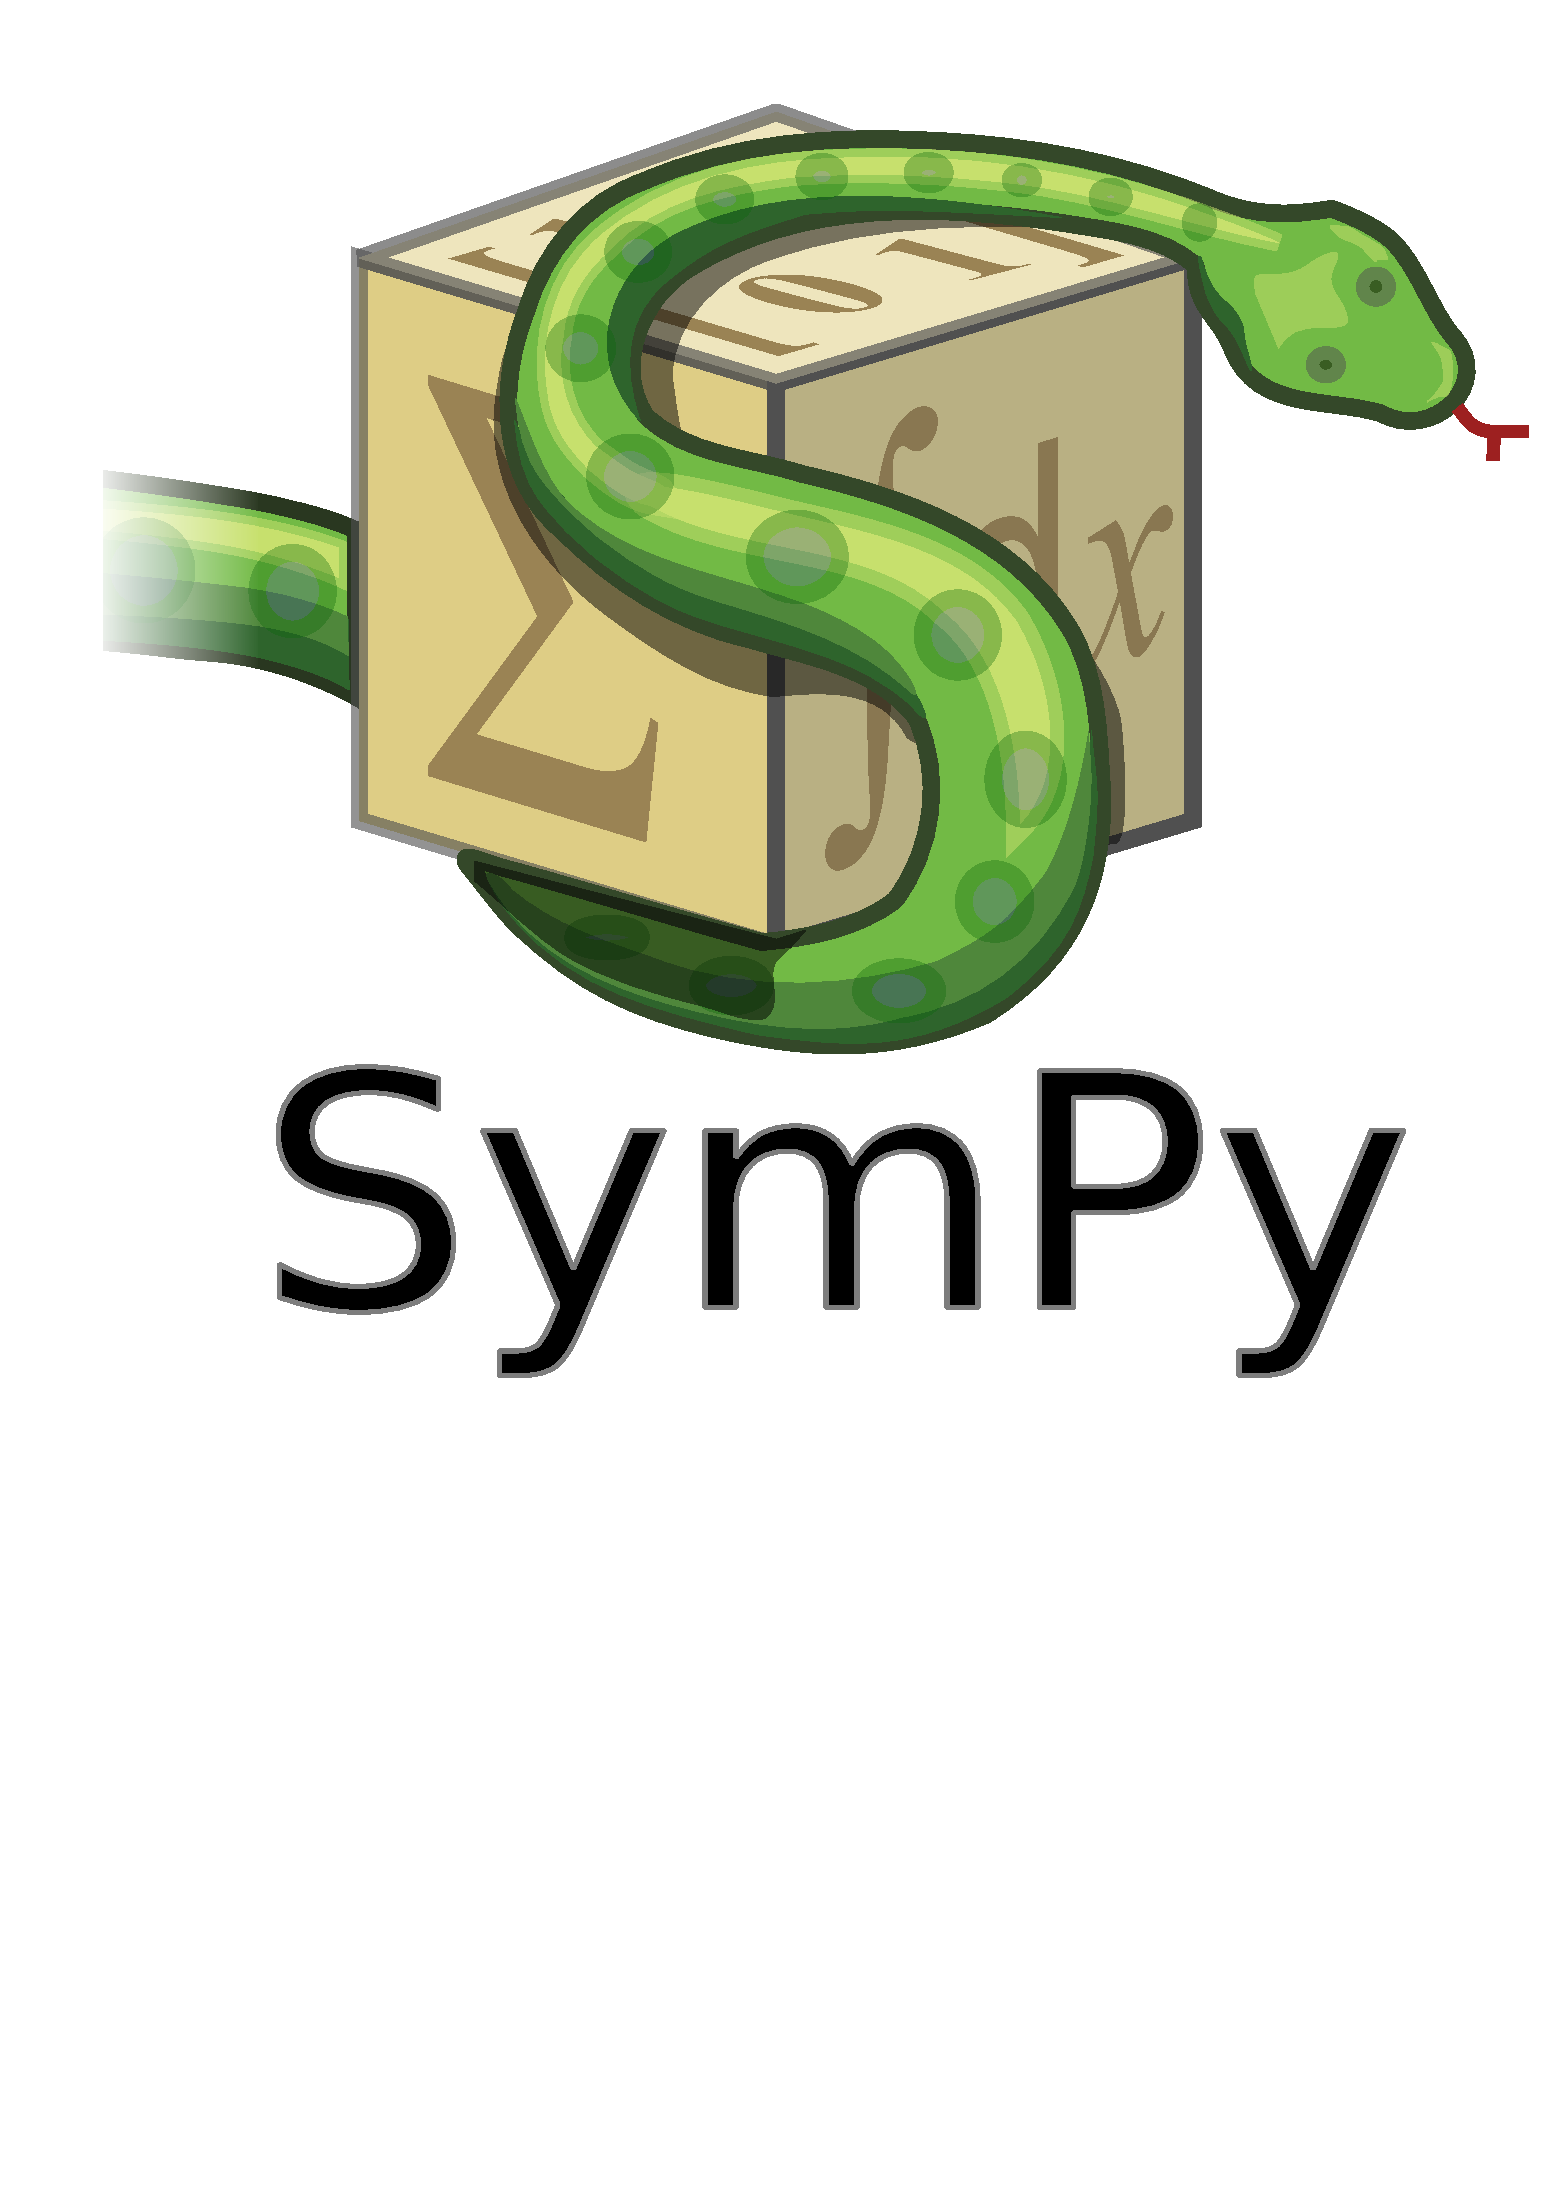
\includegraphics[scale=0.2]{images/sympy-logo.pdf}
    \end{center}
\end{frame}

\end{document}
